%----------------------------------------------------------------------------------------
%	PACKAGES AND OTHER DOCUMENT CONFIGURATIONS
%----------------------------------------------------------------------------------------

\documentclass{article}

\usepackage{fancyhdr} % Required for custom headers
\usepackage{lastpage} % Required to determine the last page for the footer
\usepackage{extramarks} % Required for headers and footers
\usepackage{graphicx}

% Margins
\topmargin=-0.45in
\evensidemargin=0in
\oddsidemargin=0in
\textwidth=6.5in
\textheight=9.0in
\headsep=0.25in

\linespread{1.1} % Line spacing

% Set up the header and footer
\pagestyle{fancy}
\lhead{\authorName} % Top left header
\chead{\pageTitle} % Top center header
\rhead{\courseName} % Top right header
\lfoot{\lastxmark} % Bottom left footer
\cfoot{} % Bottom center footer
\rfoot{Page\ \thepage\ of\ \pageref{LastPage}} % Bottom right footer
\renewcommand\headrulewidth{0.4pt} % Size of the header rule
\renewcommand\footrulewidth{0.4pt} % Size of the footer rule

%----------------------------------------------------------------------------------------
%	NAME AND CLASS SECTION
%----------------------------------------------------------------------------------------

\newcommand{\pageTitle}{Heuristic Analyis: Isolation Agent} % Assignment title
\newcommand{\courseName}{Artificial Intelligence Nanodegree} % Course/class
\newcommand{\authorName}{Johannes Stricker} % Your name

%----------------------------------------------------------------------------------------
%	TITLE PAGE
%----------------------------------------------------------------------------------------

\title{
\vspace{2in}
\textmd{\textbf{\courseName:\ \pageTitle}}\\
\normalsize\vspace{0.1in}\small{Due\ on\ \hmwkDueDate}\\
\vspace{0.1in}\large{\textit{\hmwkClassInstructor\ \hmwkClassTime}}
\vspace{3in}
}

\author{\textbf{\authorName}}
\date{} % Insert date here if you want it to appear below your name

%----------------------------------------------------------------------------------------

\begin{document}

\section{Heuristic Analysis}
Several heuristic score functions have been examined in the process of the heuristic
analysis. Therefore 500.000 games between two players choosing random moves have been
sampled to look at the correlation between the sums of the individual score functions
over complete games and the win-percentage in those games.
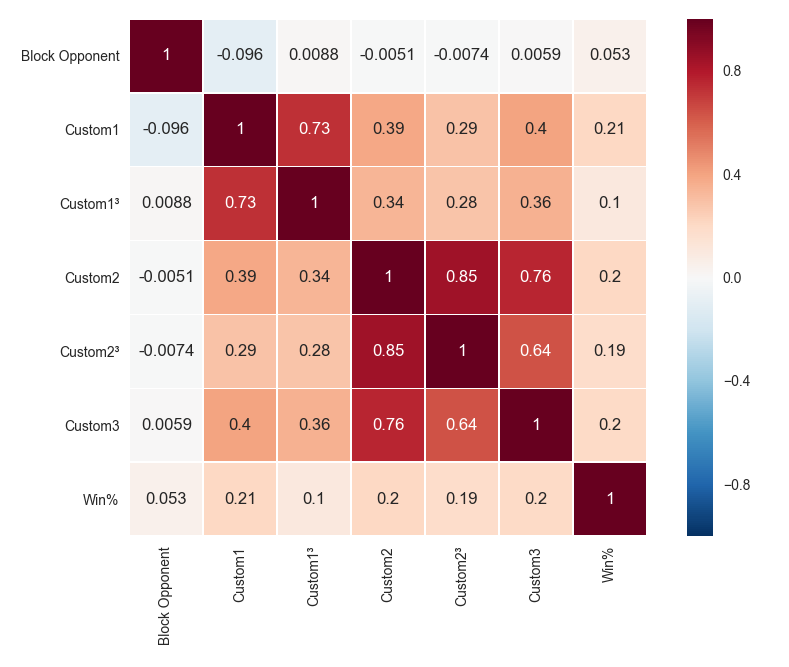
\includegraphics[width=\textwidth]{./correlation.png}
Several more functions have been examined, as well as combinations of those functions,
but describing every single function would go beyond the scope of this paper.
The three best performing functions are presented in detail below. For brevity we will refer
to the acting player as 'hero' and to his opponent as 'villain' in the function
descriptions.

\subsection{Custom$_1$}
Returns the difference between the number of available moves to hero and twice the
number of available moves to villain. The number of villain's moves is multiplied
by two, in order to punish him harder for having zero available moves. This function
intuitively makes sense, because it accurately describes hero's goal of the game: minimizing
villains moves while still being able to move himself. It has had the best overall
performance wth a 70.9\% win rate and therefore has been chosen as the primary score function.

\subsection{Custom$_2$}
Returns the difference between hero's squared distance to the board's center and villain's
squared distance to the center. In general we have most options to maneuver the board when
we occupy the center square, which is why this seems to be a reasonable heuristic to test.
With a 66.1\% win rate it scored only a little worse than than the 1st score function and this could be due to
variance, however based on the knowledge we have it seems reasonable to choose this as
the secondary score function.

\subsection{Custom$_3$}
Returns a score that describes how much either player has been pushed onto one side of the
board. It is calculated by first checking if both players are positioned on any same side
of the board and if so, the distance to the boards center for the player closest to it is
taken. This function tries to mimic the strategy of pushing a player to one side of the board.
However since players don't move in straight lines, but in an L-shape instead, this is harder
to do, which is probably why this function did not perform as well as was hoped. With 65\% it
performed worst among the three chosen score functions. It is also less comprehensable and
therefore ranks third.

\subsection{Results}
The Alphabeta agent has been tested in a tournament with each of the score heuristics
against seven other players. There have been 100 fair matches against each of those
agents. The results are presented below.

\begin{center}
  \begin{tabular}{ | l || c | c | c | }
    \hline
                     & Custom_1     & Custom_2      & Custom_3    \\ \hline
                     & Win / Loose  & Win / Loose   & Win / Loose \\ \hline \hline
      Random         & 187 / 13     & 183 / 17      & 186 / 14    \\ \hline
      MM Open        & 155 / 45     & 140 / 60      & 138 / 62    \\ \hline
      MM Center      & 185 / 15     & 166 / 34      & 164 / 36    \\ \hline
      MM Improved    & 142 / 58     & 141 / 59      & 133 / 67    \\ \hline
      AB Open        & 105 / 95     & 94 / 106      & 92 / 108    \\ \hline
      AB Center      & 119 / 81     & 104 / 96      & 105 / 95    \\ \hline
      AB Improved    & 99 / 101     & 98 / 102      & 92 / 108    \\ \hline \hline
      Win Rate       & 70.9\%       & 66.1\%        & 65.0\%      \\ \hline
  \end{tabular}
\end{center}

As mentioned, the Custom$_1$ function had the best results against all agents. It only ties against
'AB Improved', because that agent uses the same scoring heuristic. It is also a very simple to understand,
yet meaningful heuristic, since it reflects the overall goal of the game.
That's why it is the recommended scoring function.

\subsection{Conclusion}
The overall performance looks promising with a $70.9\%$ win rate for the best agent,
however if we look at the performance against other alpha-beta agents, we perform
just slightly better than $50\%$, which could probably be improved upon in some way.
However, during the analysis no combination of score functions could be found that
outperformed the difference in the available number of player moves.

\end{document}
